
\vfill

\begin{center}
{\large \textbf{Измерение цифровым вольтметром напряжения, задаваемого по стрелочному прибору}}
\end{center}

\vspace{0.5cm}

\textbf{Введение}

Основными задачами лабораторной работы являются:
\begin{enumerate}
    \item Освоение методики использования измерительного прибора для многократного прямого измерения физической величины.
    \item Выполнение элементарной статистической обработки серии результатов наблюдений при прямых измерениях.
\end{enumerate}

\begin{figure}[ht!]
\centering
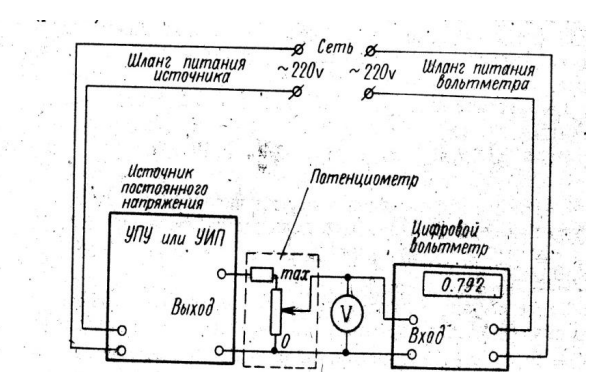
\includegraphics[width=0.7\textwidth]{Схема установки.png}
\caption{Схема лабораторной установки}
\label{fig:setup}
\end{figure}

\subsection*{Грубые измерения}

\textbf{Вычисление погрешности прибора $\Delta U_{\text{приб}}$:}

\[
\Delta U_{\text{приб}} = \frac{\delta \cdot U_{\text{ср}}}{100\%}
\]

\[
\delta = \pm \left(0,05 + 0,05 \frac{U_k}{U_{\text{ср}}}\right)\% = \frac{\Delta U_{\text{приб}}}{U_{\text{ср}}} \cdot 100\%
\]

\[
U_{\text{ср}} = \frac{\sum U_i}{n}
\]

где:
\begin{itemize}
    \item $\delta$ — относительная погрешность измерения в $\%$;
    \item $U_k$ — конечное значение установленного предела измерений;
    \item для грубых измерений $U_k = 10$ В;
    \item для точных измерений $U_k = 1$ В.
\end{itemize}

\begin{table}[ht!]
\centering
\caption{Измерения на грубой шкале}
\label{tabl:1}
\begin{tabular}{|c|c|c|c|c|}
\hline
\begin{minipage}{7mm}
    № п.п. 
\end{minipage}&
\begin{minipage}{5cm}
    Диапазон показаний использованной шкалы прибора
\end{minipage} &
\begin{minipage}{5cm}
    Результаты отдельных наблюдений ($U_i$)
\end{minipage} &
\begin{minipage}{5cm}
    Погрешность прибора на данной шкале ($\Delta U_{\text{приб}}$)
\end{minipage}\\
\hline
{}&В&В&В\\
\hline
1 &	0-10  &	0.362 & 0.0052 \\
2 &	0-10  &	0.363	& 0.0052 \\
3 &	0-10  &	0.361	& 0.0052 \\
4 &	0-10  &	0.361 & 0.0052 \\
5 & 0-10  &	0.362 & 0.0052 \\
6 & 0-10  &	0.360 & 0.0052 \\
7 & 0-10  &	0.362 & 0.0052 \\
8 & 0-10  &	0.360 & 0.0052 \\
9 & 0-10  &	0.360 & 0.0052 \\
10& 0-10  &	0.362 & 0.0052 \\
\hline
\end{tabular}
\end{table}





% Здесь может быть ваш текст перед таблицей
% ...



\clearpage
\begin{longtable}{|c|p{3.2cm}|p{3.5cm}|p{3.5cm}|}
\caption{Измерения на точной шкале}
\label{tabl:2}\\
\hline
\textbf{Номер п.п.} & \textbf{Результаты отдельных наблюдений ($U_i$)} & \textbf{Случайные отклонения от среднего $d_i = U_i - \overline{U}$} & \textbf{$d_i^2 = (U_i - \overline{U})^2$} \\
\hline
 & \textbf{(В)} & \textbf{(В)} & \textbf{(В\(^2\))} \\
\hline
\endfirsthead

\hline
\textbf{Номер п.п.} & \textbf{Результаты отдельных наблюдений ($U_i$)} & \textbf{Случайные отклонения от среднего $d_i = U_i - \overline{U}$} & \textbf{$d_i^2 = (U_i - \overline{U})^2$} \\
\hline
 & \textbf{(В)} & \textbf{(В)} & \textbf{(В\(^2\))} \\
\hline
\endhead

\hline
\multicolumn{4}{|r|}{Продолжение на следующей странице} \\
\endfoot

\hline
\endlastfoot
1  & 0.3625 & 0.000636 & 4.044$\times$10$^{-7}$ \\

2  & 0.3624 & 0.000536 & 2.873$\times$10$^{-7}$ \\

3  & 0.3627 & 0.000836 & 6.989$\times$10$^{-7}$ \\

4  & 0.3609 & -0.000964 & 9.293$\times$10$^{-7}$ \\

5  & 0.3610 & -0.000864 & 7.466$\times$10$^{-7}$ \\

6  & 0.3608 & -0.001064 & 1.132$\times$10$^{-6}$ \\

7  & 0.3610 & -0.000864 & 7.466$\times$10$^{-7}$ \\

8  & 0.3608 & -0.001064 & 1.132$\times$10$^{-6}$ \\

9  & 0.3607 & -0.001164 & 1.355$\times$10$^{-6}$ \\

10 & 0.3605 & -0.001364 & 1.861$\times$10$^{-6}$ \\

11 & 0.3617 & -0.000164 & 2.690$\times$10$^{-8}$ \\

12 & 0.3620 & 0.000136 & 1.850$\times$10$^{-8}$ \\

13 & 0.3626 & 0.000736 & 5.417$\times$10$^{-7}$ \\

14 & 0.3627 & 0.000836 & 6.989$\times$10$^{-7}$ \\

15 & 0.3628 & 0.000936 & 8.761$\times$10$^{-7}$ \\

16 & 0.3620 & 0.000136 & 1.850$\times$10$^{-8}$ \\

17 & 0.3626 & 0.000736 & 5.417$\times$10$^{-7}$ \\

18 & 0.3625 & 0.000636 & 4.044$\times$10$^{-7}$ \\

19 & 0.3624 & 0.000536 & 2.873$\times$10$^{-7}$ \\

20 & 0.3621 & 0.000236 & 5.570$\times$10$^{-8}$ \\

21 & 0.3623 & 0.000436 & 1.901$\times$10$^{-7}$ \\

22 & 0.3620 & 0.000136 & 1.850$\times$10$^{-8}$ \\

23 & 0.3618 & -0.000064 & 4.096$\times$10$^{-9}$ \\

24 & 0.3617 & -0.000164 & 2.690$\times$10$^{-8}$ \\

25 & 0.3620 & 0.000136 & 1.850$\times$10$^{-8}$ \\

26 & 0.3619 & 0.000036 & 1.296$\times$10$^{-9}$ \\

27 & 0.3614 & -0.000464 & 2.153$\times$10$^{-7}$ \\

28 & 0.3608 & -0.001064 & 1.132$\times$10$^{-6}$ \\

29 & 0.3607 & -0.001164 & 1.355$\times$10$^{-6}$ \\

30 & 0.3605 & -0.001364 & 1.861$\times$10$^{-6}$ \\

31 & 0.3608 & -0.001064 & 1.132$\times$10$^{-6}$ \\

32 & 0.3607 & -0.001164 & 1.355$\times$10$^{-6}$ \\

33 & 0.3608 & -0.001064 & 1.132$\times$10$^{-6}$ \\

34 & 0.3613 & -0.000564 & 3.181$\times$10$^{-7}$ \\

35 & 0.3623 & 0.000436 & 1.901$\times$10$^{-7}$ \\

36 & 0.3620 & 0.000136 & 1.850$\times$10$^{-8}$ \\

37 & 0.3618 & -0.000064 & 4.096$\times$10$^{-9}$ \\

38 & 0.3622 & 0.000336 & 1.129$\times$10$^{-7}$ \\

39 & 0.3620 & 0.000136 & 1.850$\times$10$^{-8}$ \\

40 & 0.3623 & 0.000436 & 1.901$\times$10$^{-7}$ \\

41 & 0.3627 & 0.000836 & 6.989$\times$10$^{-7}$ \\

42 & 0.3628 & 0.000936 & 8.761$\times$10$^{-7}$ \\

43 & 0.3622 & 0.000336 & 1.129$\times$10$^{-7}$ \\

44 & 0.3623 & 0.000436 & 1.901$\times$10$^{-7}$ \\

45 & 0.3620 & 0.000136 & 1.850$\times$10$^{-8}$ \\

46 & 0.3622 & 0.000336 & 1.129$\times$10$^{-7}$ \\
47 & 0.3620 & 0.000136 & 1.850$\times$10$^{-8}$ \\
48 & 0.3635 & 0.001636 & 2.677$\times$10$^{-6}$ \\
49 & 0.3634 & 0.001536 & 2.359$\times$10$^{-6}$ \\
50 & 0.3637 & 0.001836 & 3.371$\times$10$^{-6}$ \\
\

\end{longtable}

\begin{table}[ht!]
\centering
\caption{Результаты статистической обработки}
\label{tab:stats}
\begin{tabular}{|c|c|c|}
\hline
\(\displaystyle \overline{U} = \frac{\sum_{i=1}^{50} U_i}{50} = 0.361864 \, \text{B}\) & 
\(\displaystyle \sum_{i=1}^{50} |d_i| = 0.027456 \, \text{B}\) & 
\(\displaystyle \sum_{i=1}^{50} d_i^2 = 2.845 \times 10^{-5} \, \text{B}^2\) \\
\hline
\end{tabular}
\end{table}

\subsubsection{Графики}

\begin{figure}[ht!]
\centering
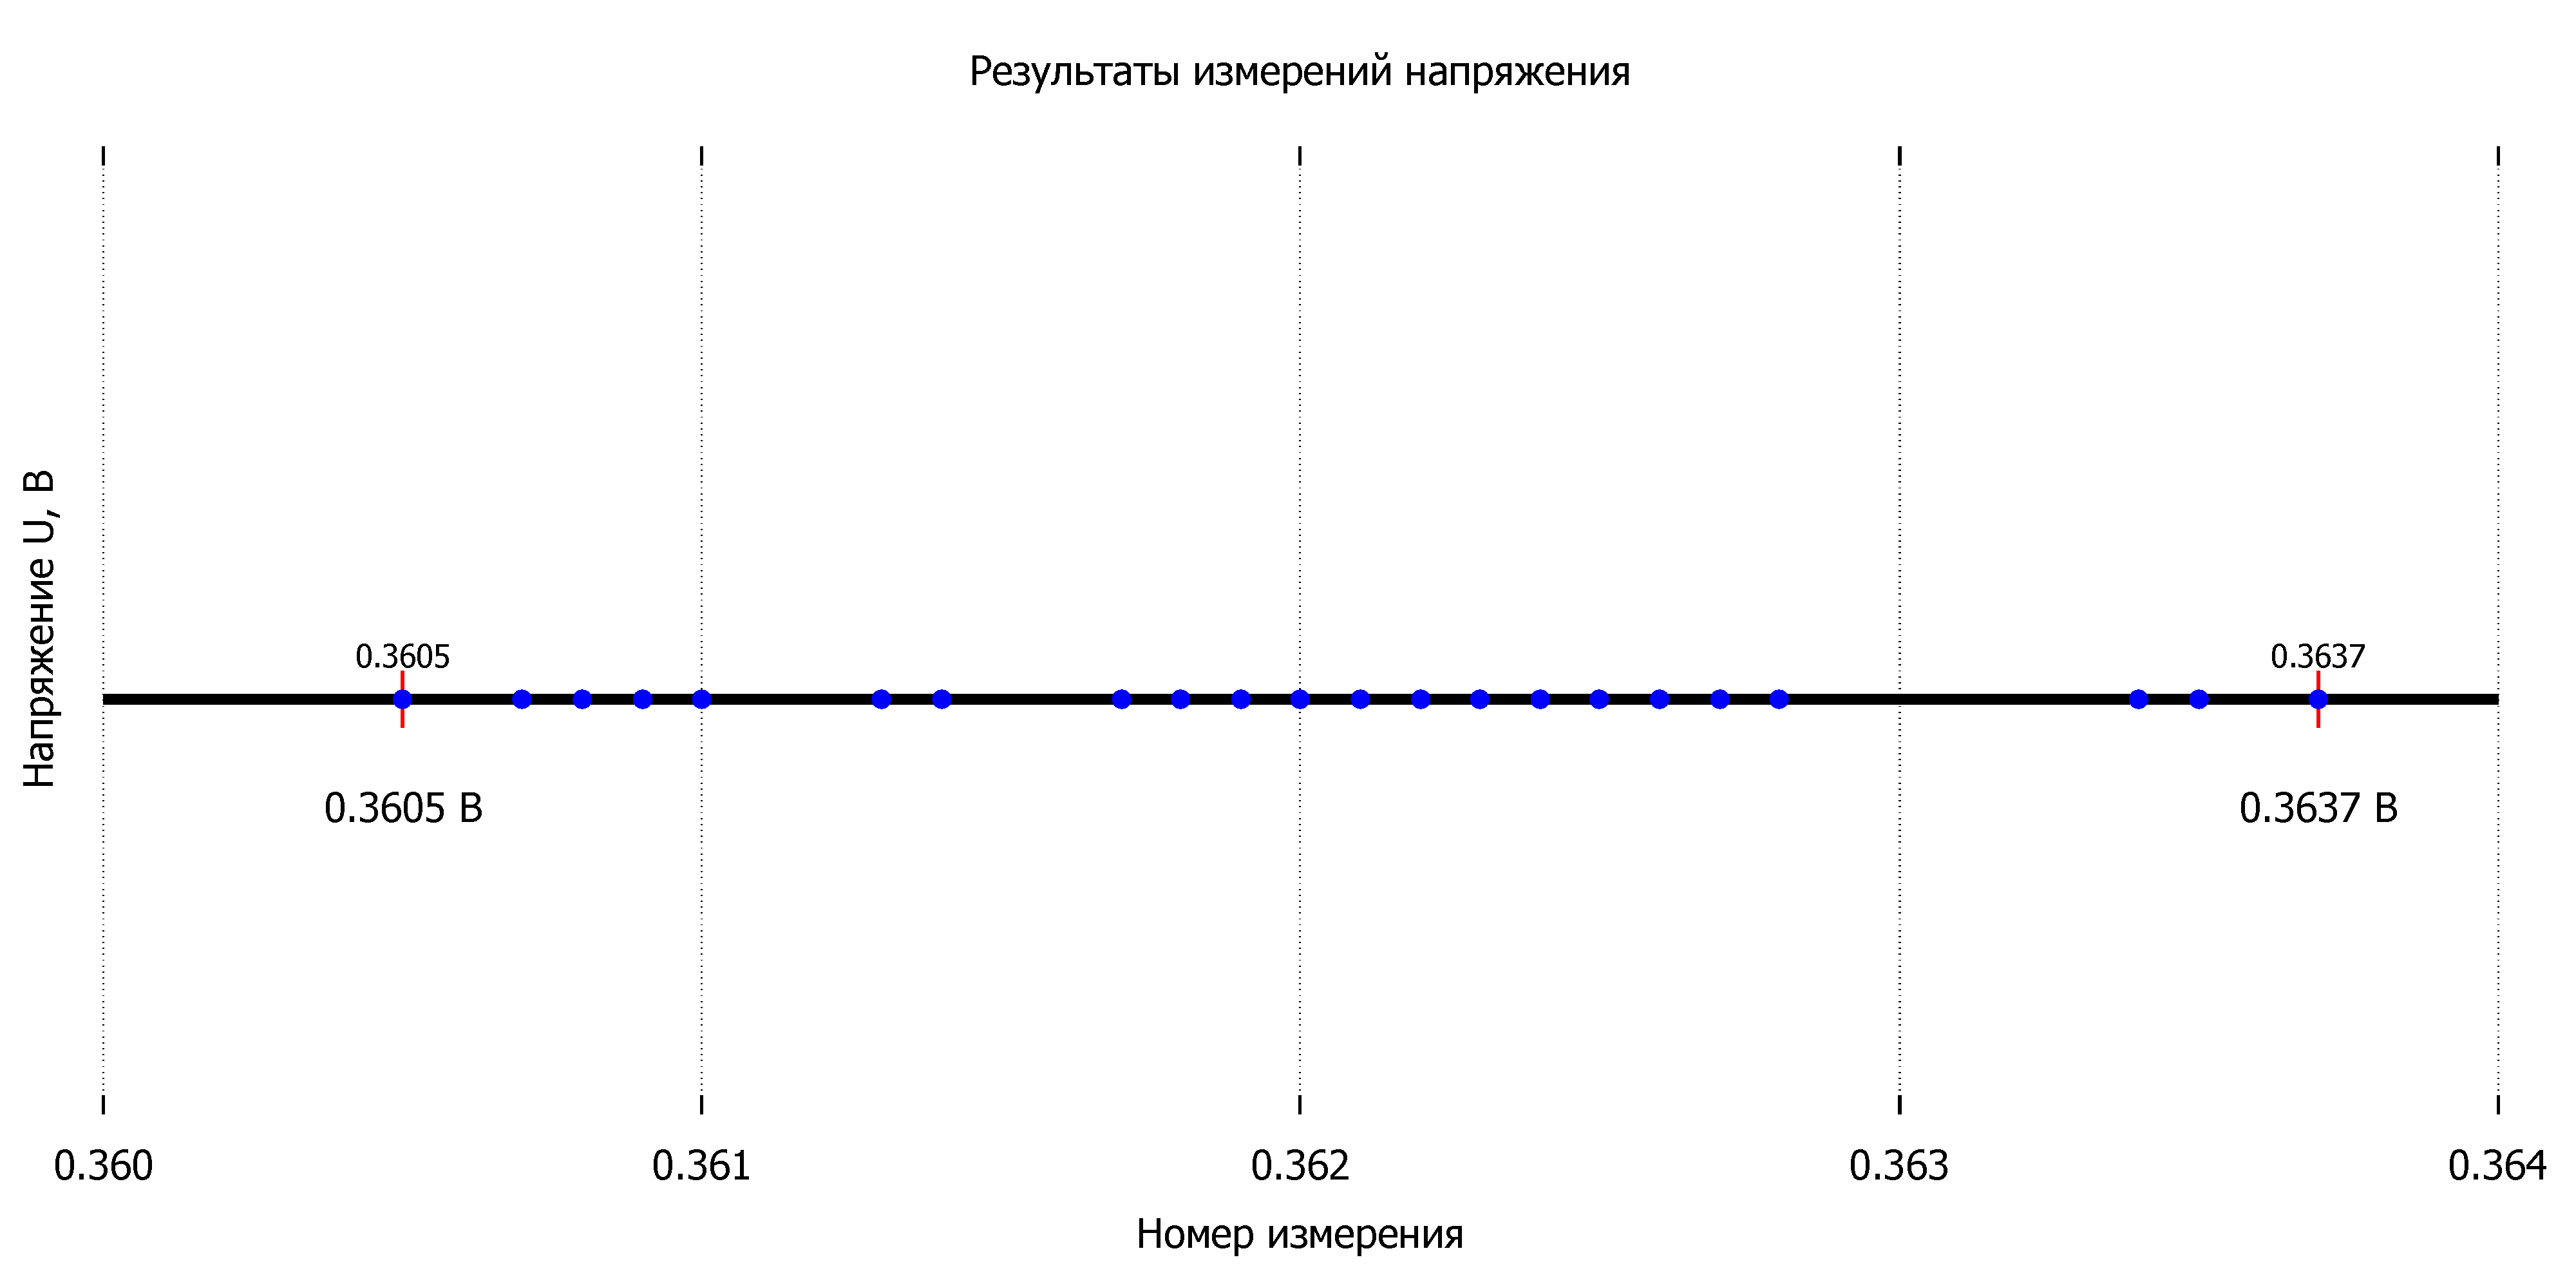
\includegraphics[width=1.05\textwidth]{график 5.pdf}
\vspace{-1.1cm}
\caption{Распределение результатов измерений на числовой оси}
\label{fig:graph}
\vspace{0.2cm}

\begin{center}
\large
$U_{\text{min}} = 0.3605$ В, \quad $U_{\text{max}} = 0.3637$ В
\end{center}
\end{figure}


\begin{figure}[H]
\centering
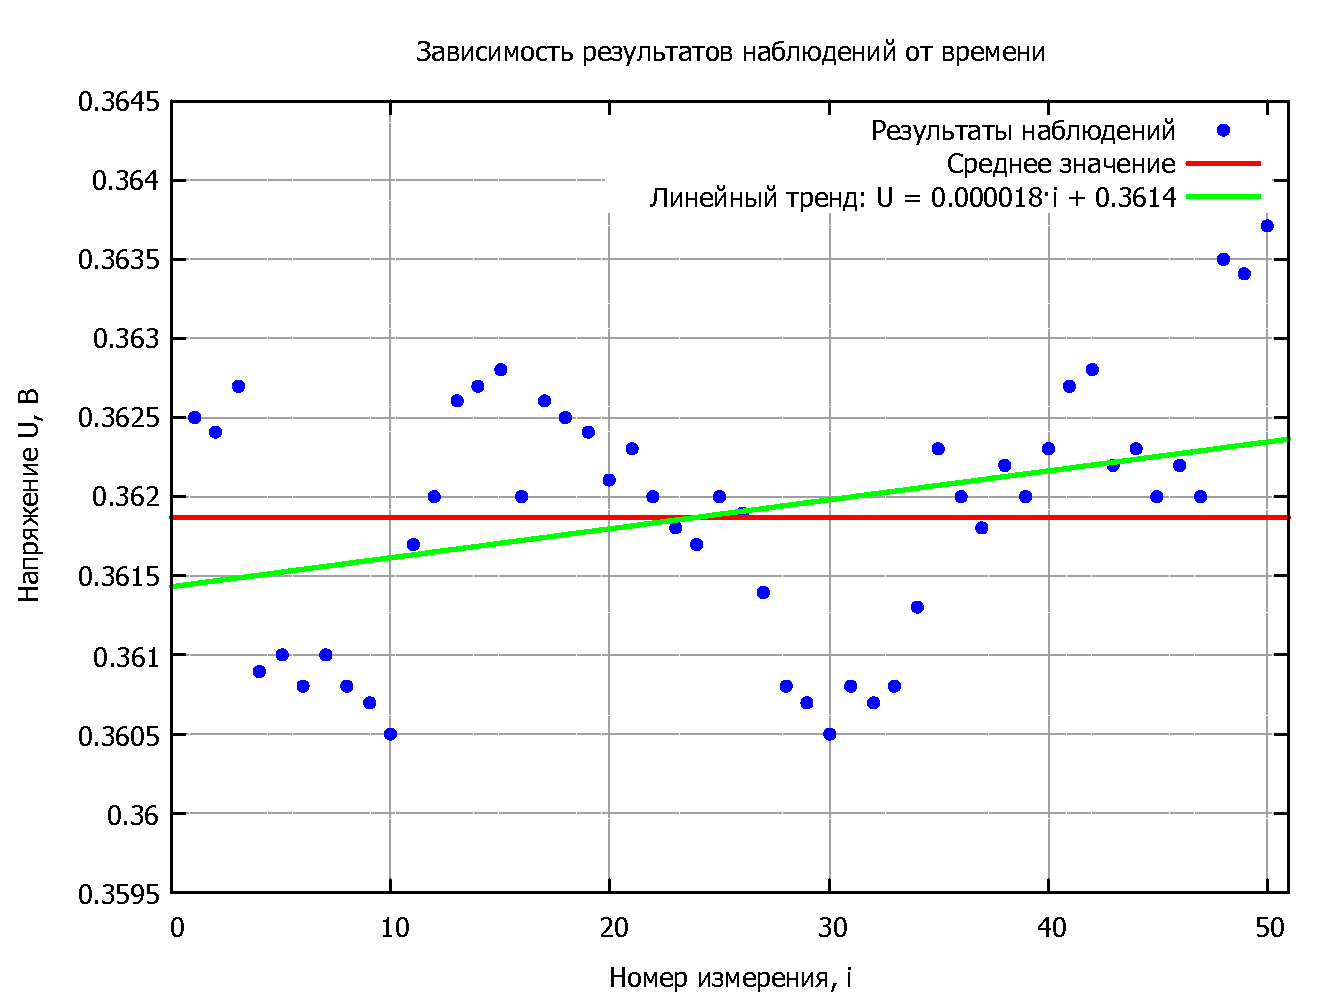
\includegraphics[width=0.8\textwidth]{График ПДФ.pdf}
\caption{Зависимость результатов наблюдений от времени}
\label{fig:drift}
\end{figure}


\clearpage
\subsection*{Таблица 4. Распределение результатов измерений по интервалам}

\begin{table}[ht!]
\centering
\label{tab:histogram}
\begin{tabular}{|c|c|c|c|}
\hline
\textbf{№} & \textbf{Границы интервала (В)} & \textbf{Частота} & \textbf{Доля} \\
\hline
1 & 0.3605--0.3608 & 5 & 0.10 \\
\hline
2 & 0.3608--0.3611 & 4 & 0.08 \\
\hline
3 & 0.3611--0.3615 & 2 & 0.04 \\
\hline
4 & 0.3615--0.3618 & 3 & 0.06 \\
\hline
5 & 0.3618--0.3621 & 9 & 0.18 \\
\hline
6 & 0.3621--0.3624 & 8 & 0.16 \\
\hline
7 & 0.3624--0.3627 & 8 & 0.16 \\
\hline
8 & 0.3627--0.3631 & 5 & 0.10 \\
\hline
9 & 0.3631--0.3634 & 2 & 0.04 \\
\hline
10 & 0.3634--0.3637 & 4 & 0.08 \\
\hline
\multicolumn{3}{|c|}{\textbf{Сумма}} & \textbf{1.00} \\
\hline
\end{tabular}
\end{table}

\vspace{0.5cm}
\begin{figure}[ht!]
\centering
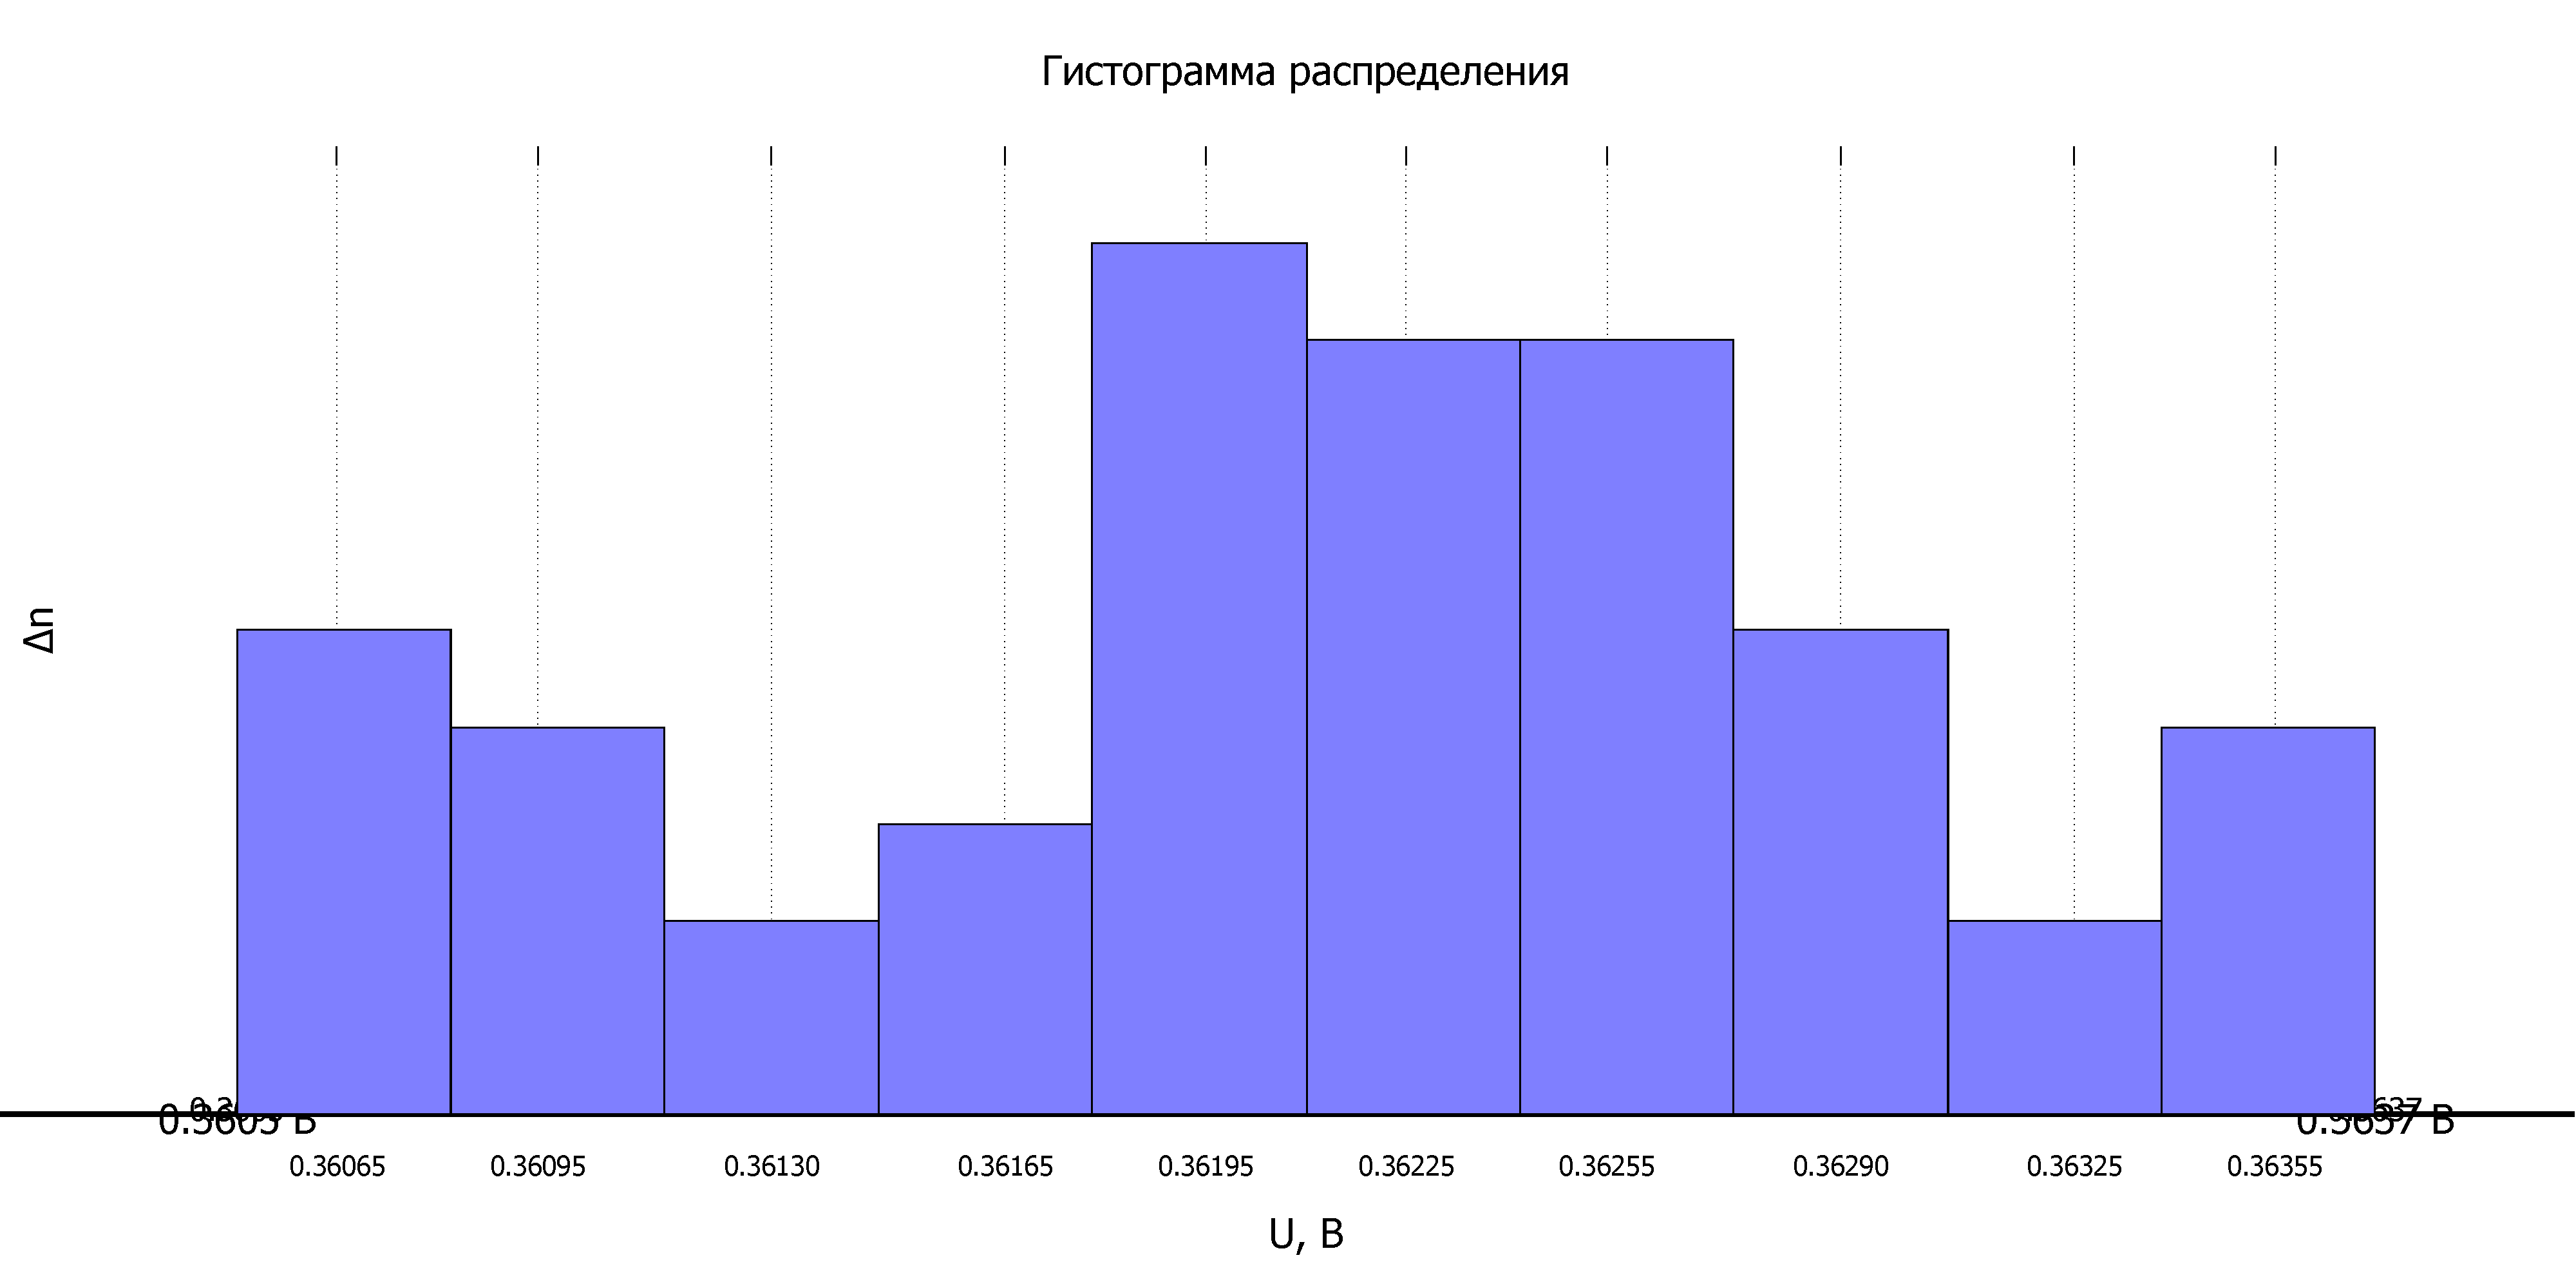
\includegraphics[width=1.0\textwidth]{гистограмма 1.pdf}
\caption{Гистограмма распределения результатов измерений}
\label{fig:histogram}
\end{figure}




\clearpage
\begin{figure}[ht!]
\centering
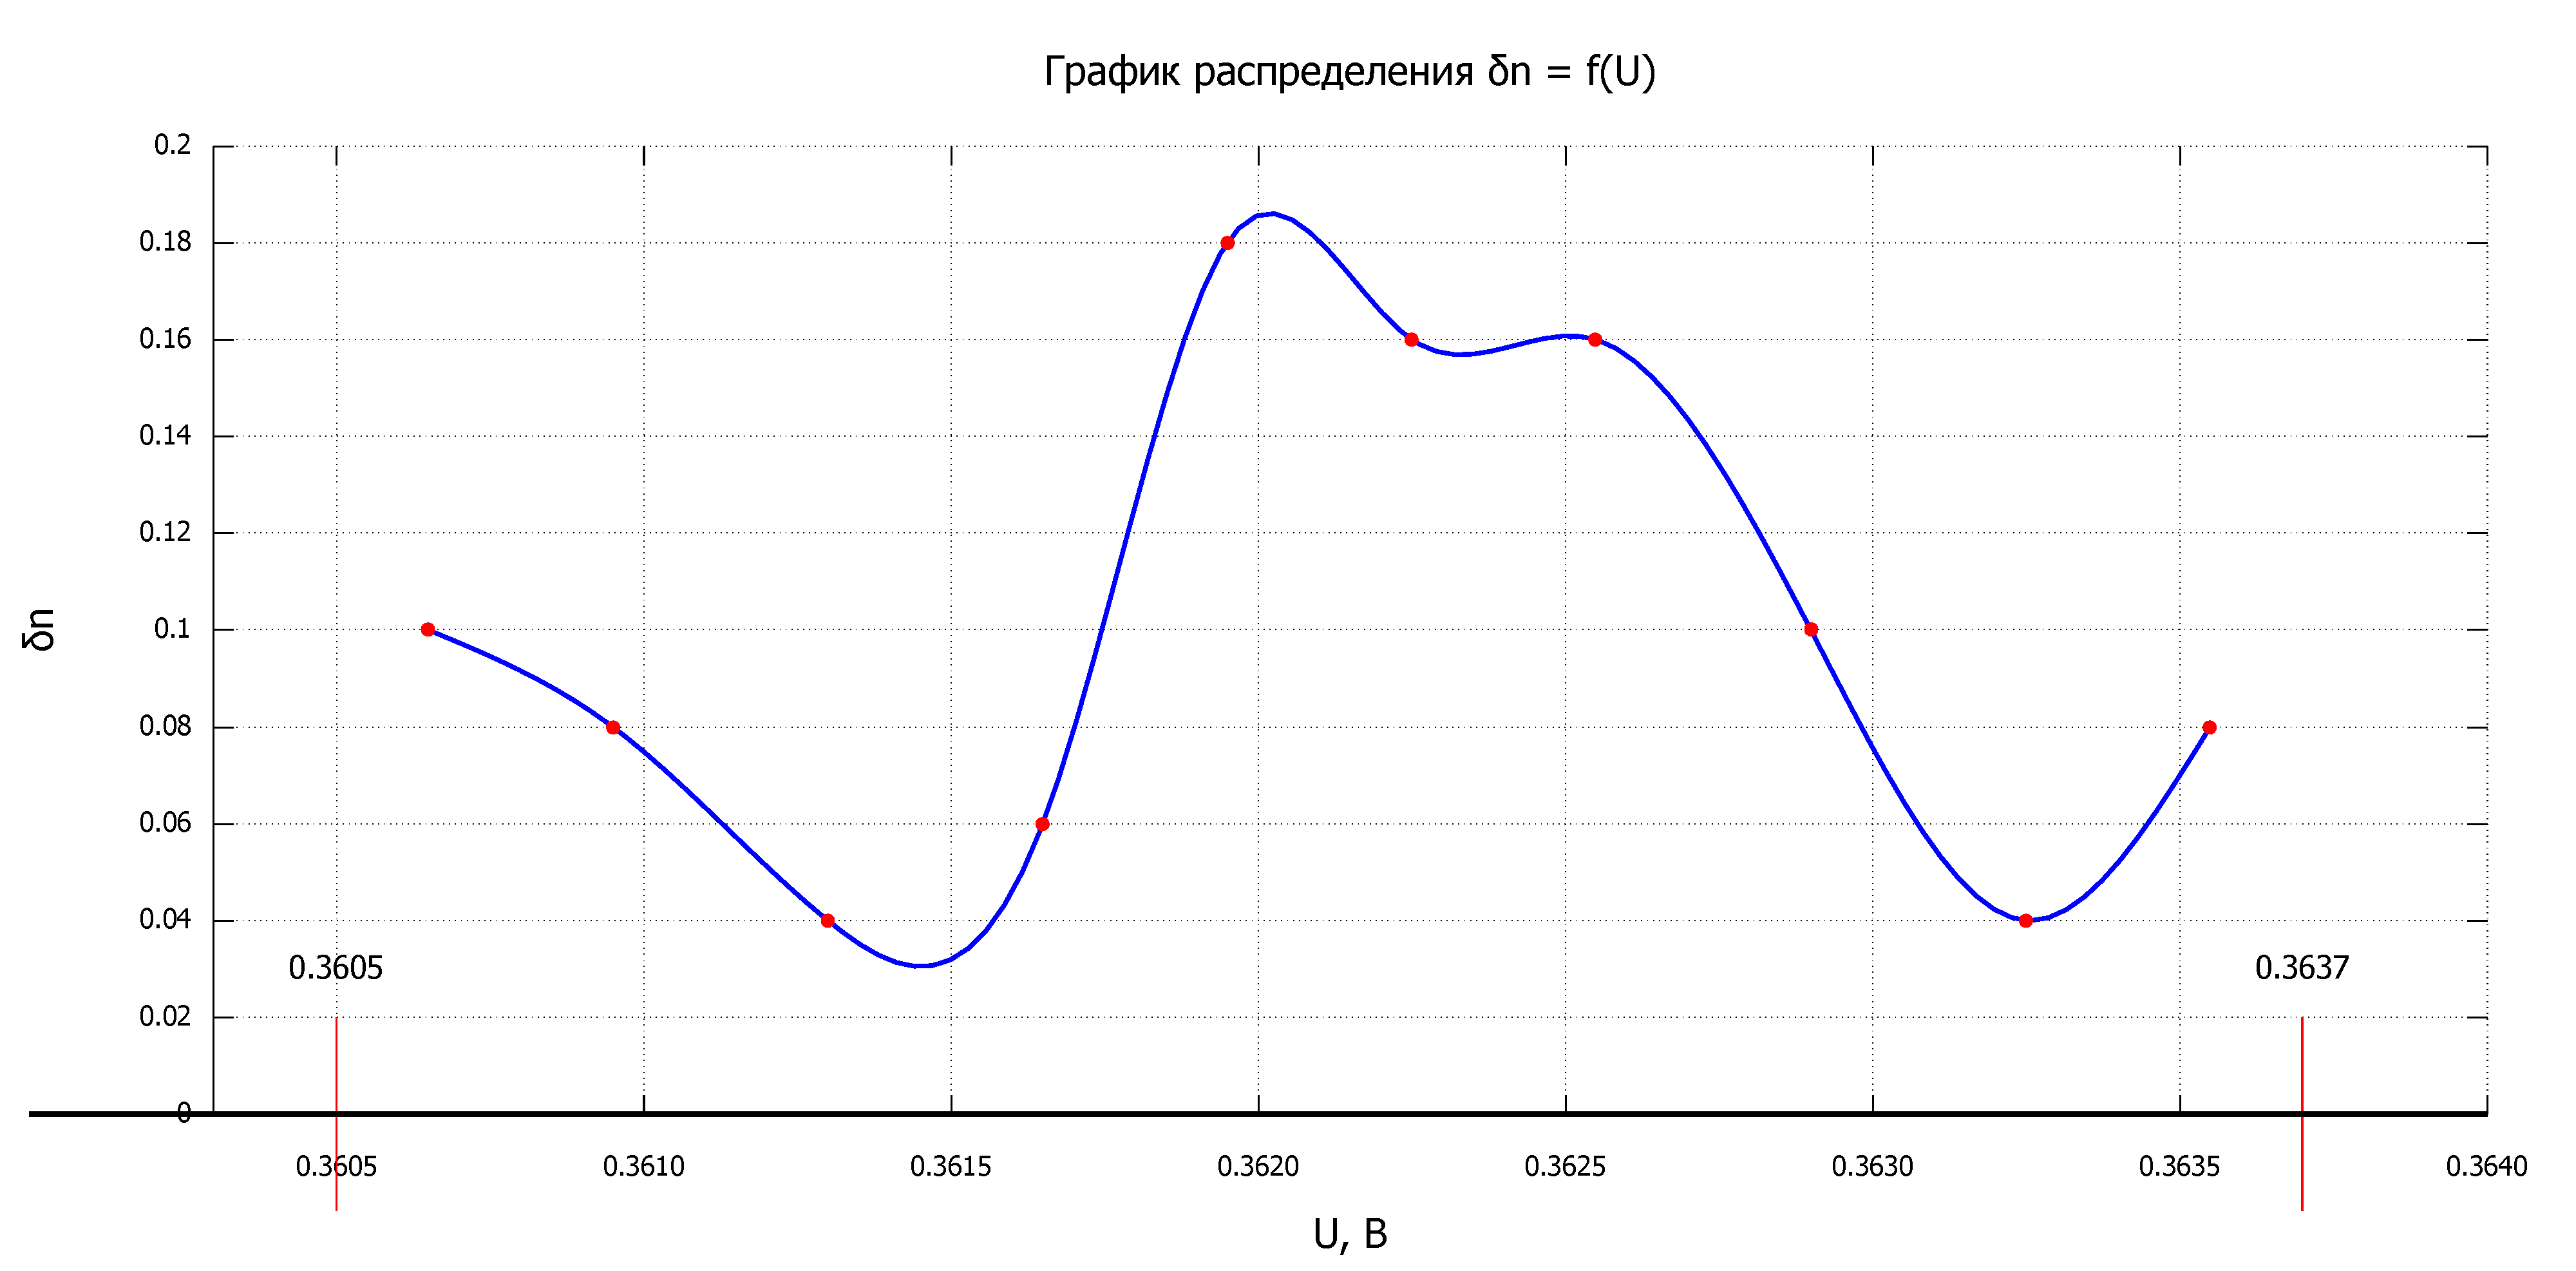
\includegraphics[width=1.0\textwidth]{распр 1.pdf}
\vspace{-0.8cm}
\caption{График распределения $\delta n = f(U)$}
\label{fig:distribution}
\end{figure}

\vspace{0.5cm}
\subsection*{Статистическая обработка результатов}

Дисперсия:
\[
\sigma^2 = \frac{1}{n-1}\sum_{i=1}^{50} (U_i - \overline{U})^2 \approx 5.806 \times 10^{-7} \, \text{В}^2
\]

Среднеквадратичное отклонение:
\[
\sigma = \sqrt{\sigma^2} \approx 0.000762 \, \text{В}
\]

Средняя квадратичная погрешность среднего:
\[
\Delta U = \frac{\sigma}{\sqrt{n}} = \frac{0.000762}{\sqrt{50}} \approx 0.000108 \, \text{В}
\]

Окончательный результат:
\[
U = \overline{U} \pm \Delta U = 0.361864 \pm 0.000108 \, \text{В}
\]





\section*{Выводы}
В результате проделанной работы я познакомился с методиками использования измерительного прибора для многократного прямого измерения физической величины на примере работы с установкой для измерения напряжения цифровым вольтметром, научился выполнять простую статистическую обработку серии результатов наблюдений при прямых измерениях (с вычислением дисперсии и среднеквадратичным отклонением).
